\documentclass[a4paper,11pt]{article}

% ───────────────────────────
%         PACKAGES
% ───────────────────────────
\usepackage[utf8]{inputenc}
\usepackage[T1]{fontenc}
\usepackage{geometry}
\usepackage{graphicx}
\usepackage{amsmath, amssymb}
\usepackage{booktabs}
\usepackage{enumitem}
\usepackage{hyperref}
\usepackage{caption}
\usepackage{subcaption}
\usepackage{float}

\usepackage{fancyhdr}
\usepackage{titlesec}
\usepackage{parskip}

\usepackage{minted}
\usepackage{inconsolata}  % clean monospaced font
\usepackage{mathpazo}     % professional text font

\usepackage{array}
\usepackage{booktabs}
\usepackage[table]{xcolor}


% ───────────────────────────
%         GEOMETRY
% ───────────────────────────
\geometry{
	a4paper,
	left=2.5cm,
	right=2.5cm,
	top=2.5cm,
	bottom=2.5cm
}

% ───────────────────────────
%         HEADER/FOOTER
% ───────────────────────────
\pagestyle{fancy}
\fancyhf{}
\renewcommand{\headrulewidth}{0.4pt}
\renewcommand{\footrulewidth}{0.4pt}
\lhead{\textsf{\textcolor{gray}{Depth Image Processing Journal}}}
\rhead{\textsf{\textcolor{gray}{Siddharth Patel}}}
\rfoot{\textsf{\textcolor{gray}{\thepage}}}

% ───────────────────────────
%         TITLE FORMAT
% ───────────────────────────
\titleformat{\section}
{\Large\bfseries\sffamily\color{black}}
{\thesection}{1em}{}

\titleformat{\subsection}
{\large\bfseries\sffamily\color{black}}
{\thesubsection}{1em}{}

% ───────────────────────────
%         MINTED SETTINGS
% ───────────────────────────
\definecolor{mintbg}{rgb}{0.97,0.97,0.97}
\setminted{
	bgcolor=mintbg,
	fontsize=\footnotesize,
	linenos=true,
	numbersep=5pt,
	frame=lines,
	framesep=2mm,
	breaklines=true,
	tabsize=4,
	encoding=utf8
}

% ───────────────────────────
%         TITLE PAGE
% ───────────────────────────
\title{\Huge \textbf{Depth Image Processing Journal}\\[1ex]
	\Large Experiments with Python and OpenCV}
\author{\textbf{Siddharth Patel} \\ HTW Berlin}
\date{\today}

% in preamble:
\usepackage{graphicx}
\usepackage{pgffor}

% One full-page image per page (A4)
\newcommand{\FullPageImage}[2]{%
	\begin{figure}[H]
		\centering
		\includegraphics[width=0.88\textwidth,height=\textheight,keepaspectratio]{#1}%
		\caption{\texttt{#2}}% unnumbered caption, shows the name
	\end{figure}
}

% Helper: loop for each blur type
\newcommand{\PrintCannySeries}[1]{%
	\foreach[count=\n from 1] \t in {10,20,30,40,50,60,70,80,90,100,110,120,130,140,150,160,170,180,190,200,210}{%
		\pgfmathtruncatemacro{\hi}{\t*3}%
		\edef\idx{\ifnum\n<10 0\the\numexpr\n\relax\else \the\numexpr\n\relax\fi}%
		\edef\fname{images/canny_on_gray/#1_\idx_canny_\t_\hi.png}%
		\edef\name{#1\_\idx\_canny\_\t\_\hi}%
		\FullPageImage{\fname}{\name}%
	}%
}

% ───────────────────────────
%         BEGIN DOCUMENT
% ───────────────────────────
\begin{document}
	
	\maketitle
	\thispagestyle{empty}
	\newpage
	\tableofcontents
	\newpage

	
	% ───────────────────────────
	%       INTRODUCTION
	% ───────────────────────────
	\section{Introduction}
	This journal documents my experiments in depth image processing using Python and OpenCV. 
	The goal is to apply different filters and processing methods on depth frames in order 
	to eventually detect the edge of a table and retrieve the distance to it. 
	For each experiment, I will include:
	\begin{itemize}[noitemsep]
		\item The Python code used
		\item Sample output frame(s) for comparison
		\item Observations about filter performance
	\end{itemize}
	
	% ───────────────────────────
	%   SECTION 1: Experiment Setup
	% ───────────────────────────
	\section{Experiment Setup}
	
	The first step in this project is to define the experimental setup and show the position of the depth camera on the robot. 
	The robot platform is equipped with a depth sensor mounted at the front, as shown in the following images. 
	This setup will be used to capture depth frames while approaching the edge of a table, which forms the basis for the 
	subsequent image processing experiments.
	
	\begin{figure}[h!]
		\centering
		\begin{subfigure}{0.48\textwidth}
			\centering
			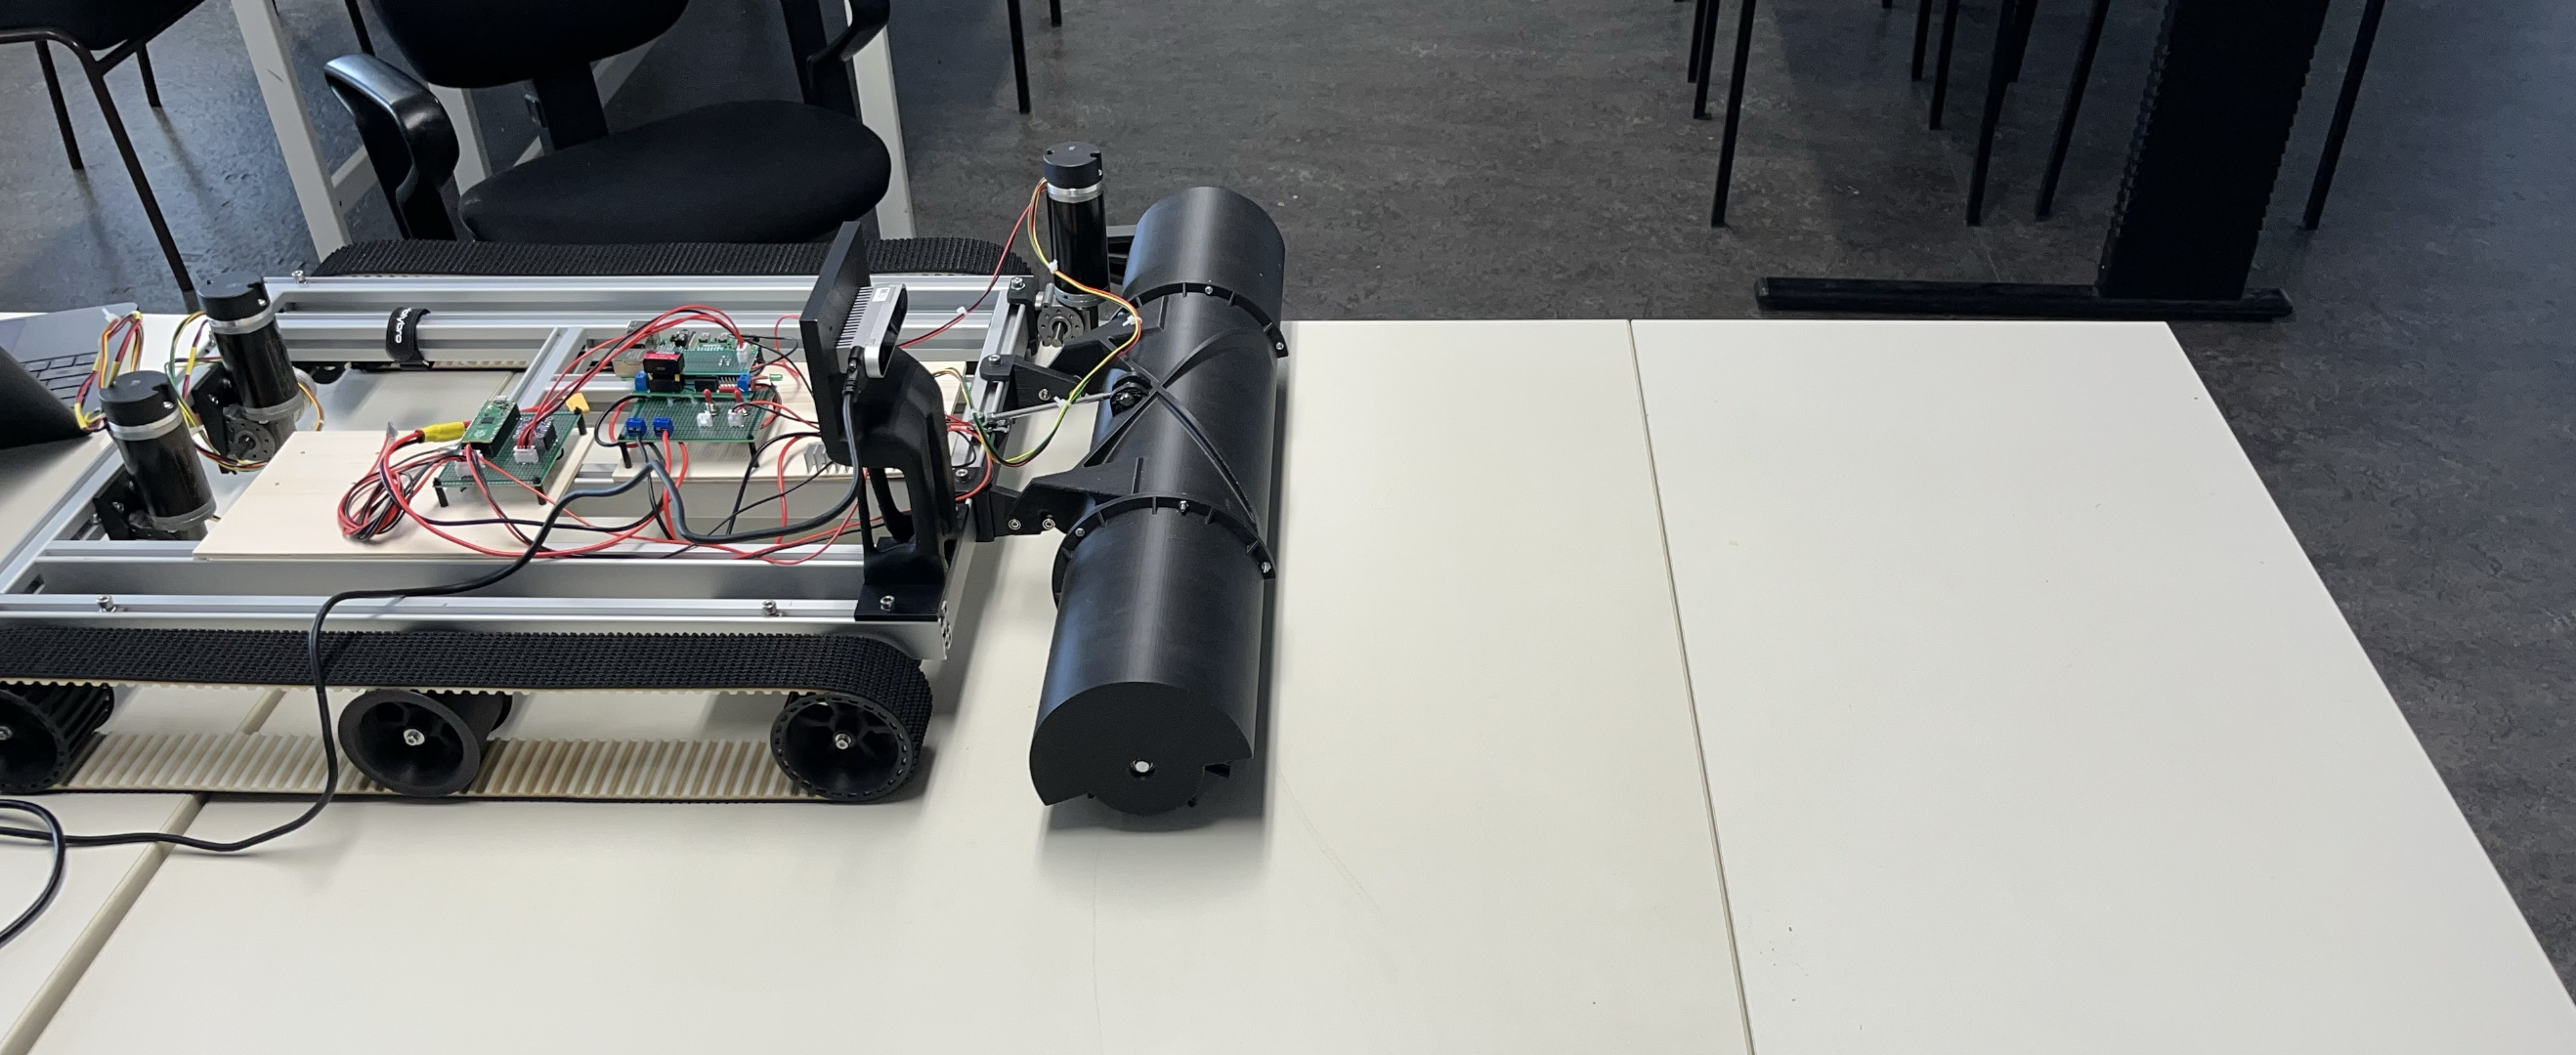
\includegraphics[width=\linewidth]{Images/setup_side.png}
			\caption{Side view of the robot with mounted depth camera.}
		\end{subfigure}\hfill
		\begin{subfigure}{0.48\textwidth}
			\centering
			\includegraphics[width=\linewidth]{Images/setup_top.png}
			\caption{Top view of the robot and camera orientation.}
		\end{subfigure}
		\caption{Experimental setup: depth camera mounted on robot platform.}
	\end{figure}
	
	% ───────────────────────────
	%   SECTION 3: Depth Frame via ROS Subscription
	% ───────────────────────────
	\section{Depth Frame Subscription (ROS)}
	
	Goal: subscribe to the depth topic and convert the ROS image to OpenCV with \texttt{cv\_bridge}.  
	We show three basic views: original depth, gray, and colored.
	
	\subsection*{Source}
	\href{http://wiki.ros.org/cv_bridge/Tutorials/ConvertingBetweenROSImagesAndOpenCVImagesPython}{cv\_bridge tutorial (Python)}
	
	\subsection{Code}
	\inputminted{python}{Python_Files/03_depth_subscription.py}
	
	\subsection{Output Frames}
	\begin{figure}[H]
		\centering
		\begin{subfigure}{0.32\textwidth}
			\centering
			
\includegraphics[width=\linewidth]{Images/depth_original.png}
			\caption{Depth Original}
		\end{subfigure}\hfill
		\begin{subfigure}{0.32\textwidth}
			\centering
			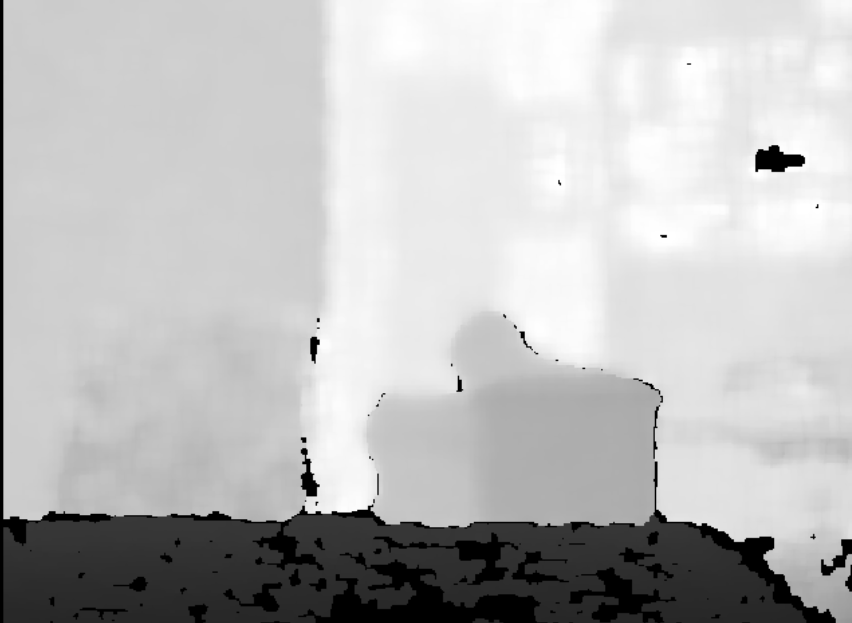
\includegraphics[width=\linewidth]{Images/depth_gray.png}
			\caption{Depth Gray}
		\end{subfigure}\hfill
			\begin{subfigure}{0.32\textwidth}
			\centering
			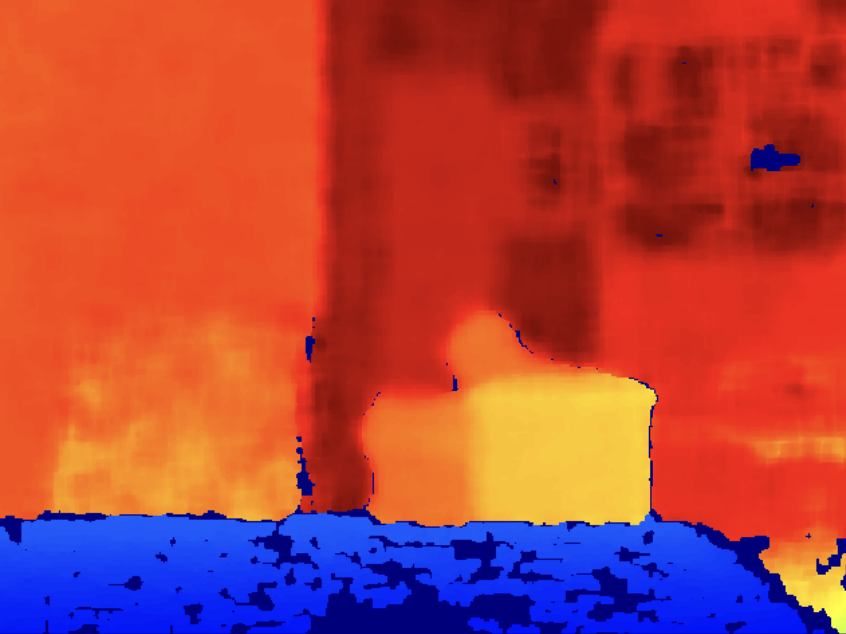
\includegraphics[width=\linewidth]{Images/depth_colored.png}
			\caption{Depth Colored}
		\end{subfigure}
		
		\caption{Three fundamental views of the same depth frame.}
	\end{figure}
	
	\subsection*{Notes}
	Original is the raw depth visualization; Gray is normalized to 8-bit; Colored uses a colormap for contrast.
	
	% ───────────────────────────
	%   SECTION 4: Image Blurring (Image Smoothing)
	% ───────────────────────────
	\section{Image Blurring (Image Smoothing)}
	
	In this section I illustrate four different blurring techniques that can be applied to depth images.  
	
	\subsection*{Source}
	\href{https://docs.opencv.org/4.x/d4/d13/tutorial_py_filtering.html}{OpenCV Documentation – Image Filtering}
	
	\subsection{Averaging}
	\subsubsection*{Code}
	\inputminted{python}{Python_Files/04_average_blur.py}
	
	% Averaging
	This blur replaces each pixel with the average of its neighboring pixels under a kernel.  
	\textbf{Use:} Simple smoothing, reduces overall noise but also blurs edges.
	

	
	\subsubsection*{Output (Gray Grid)}
	\begin{figure}[H]
		\centering
		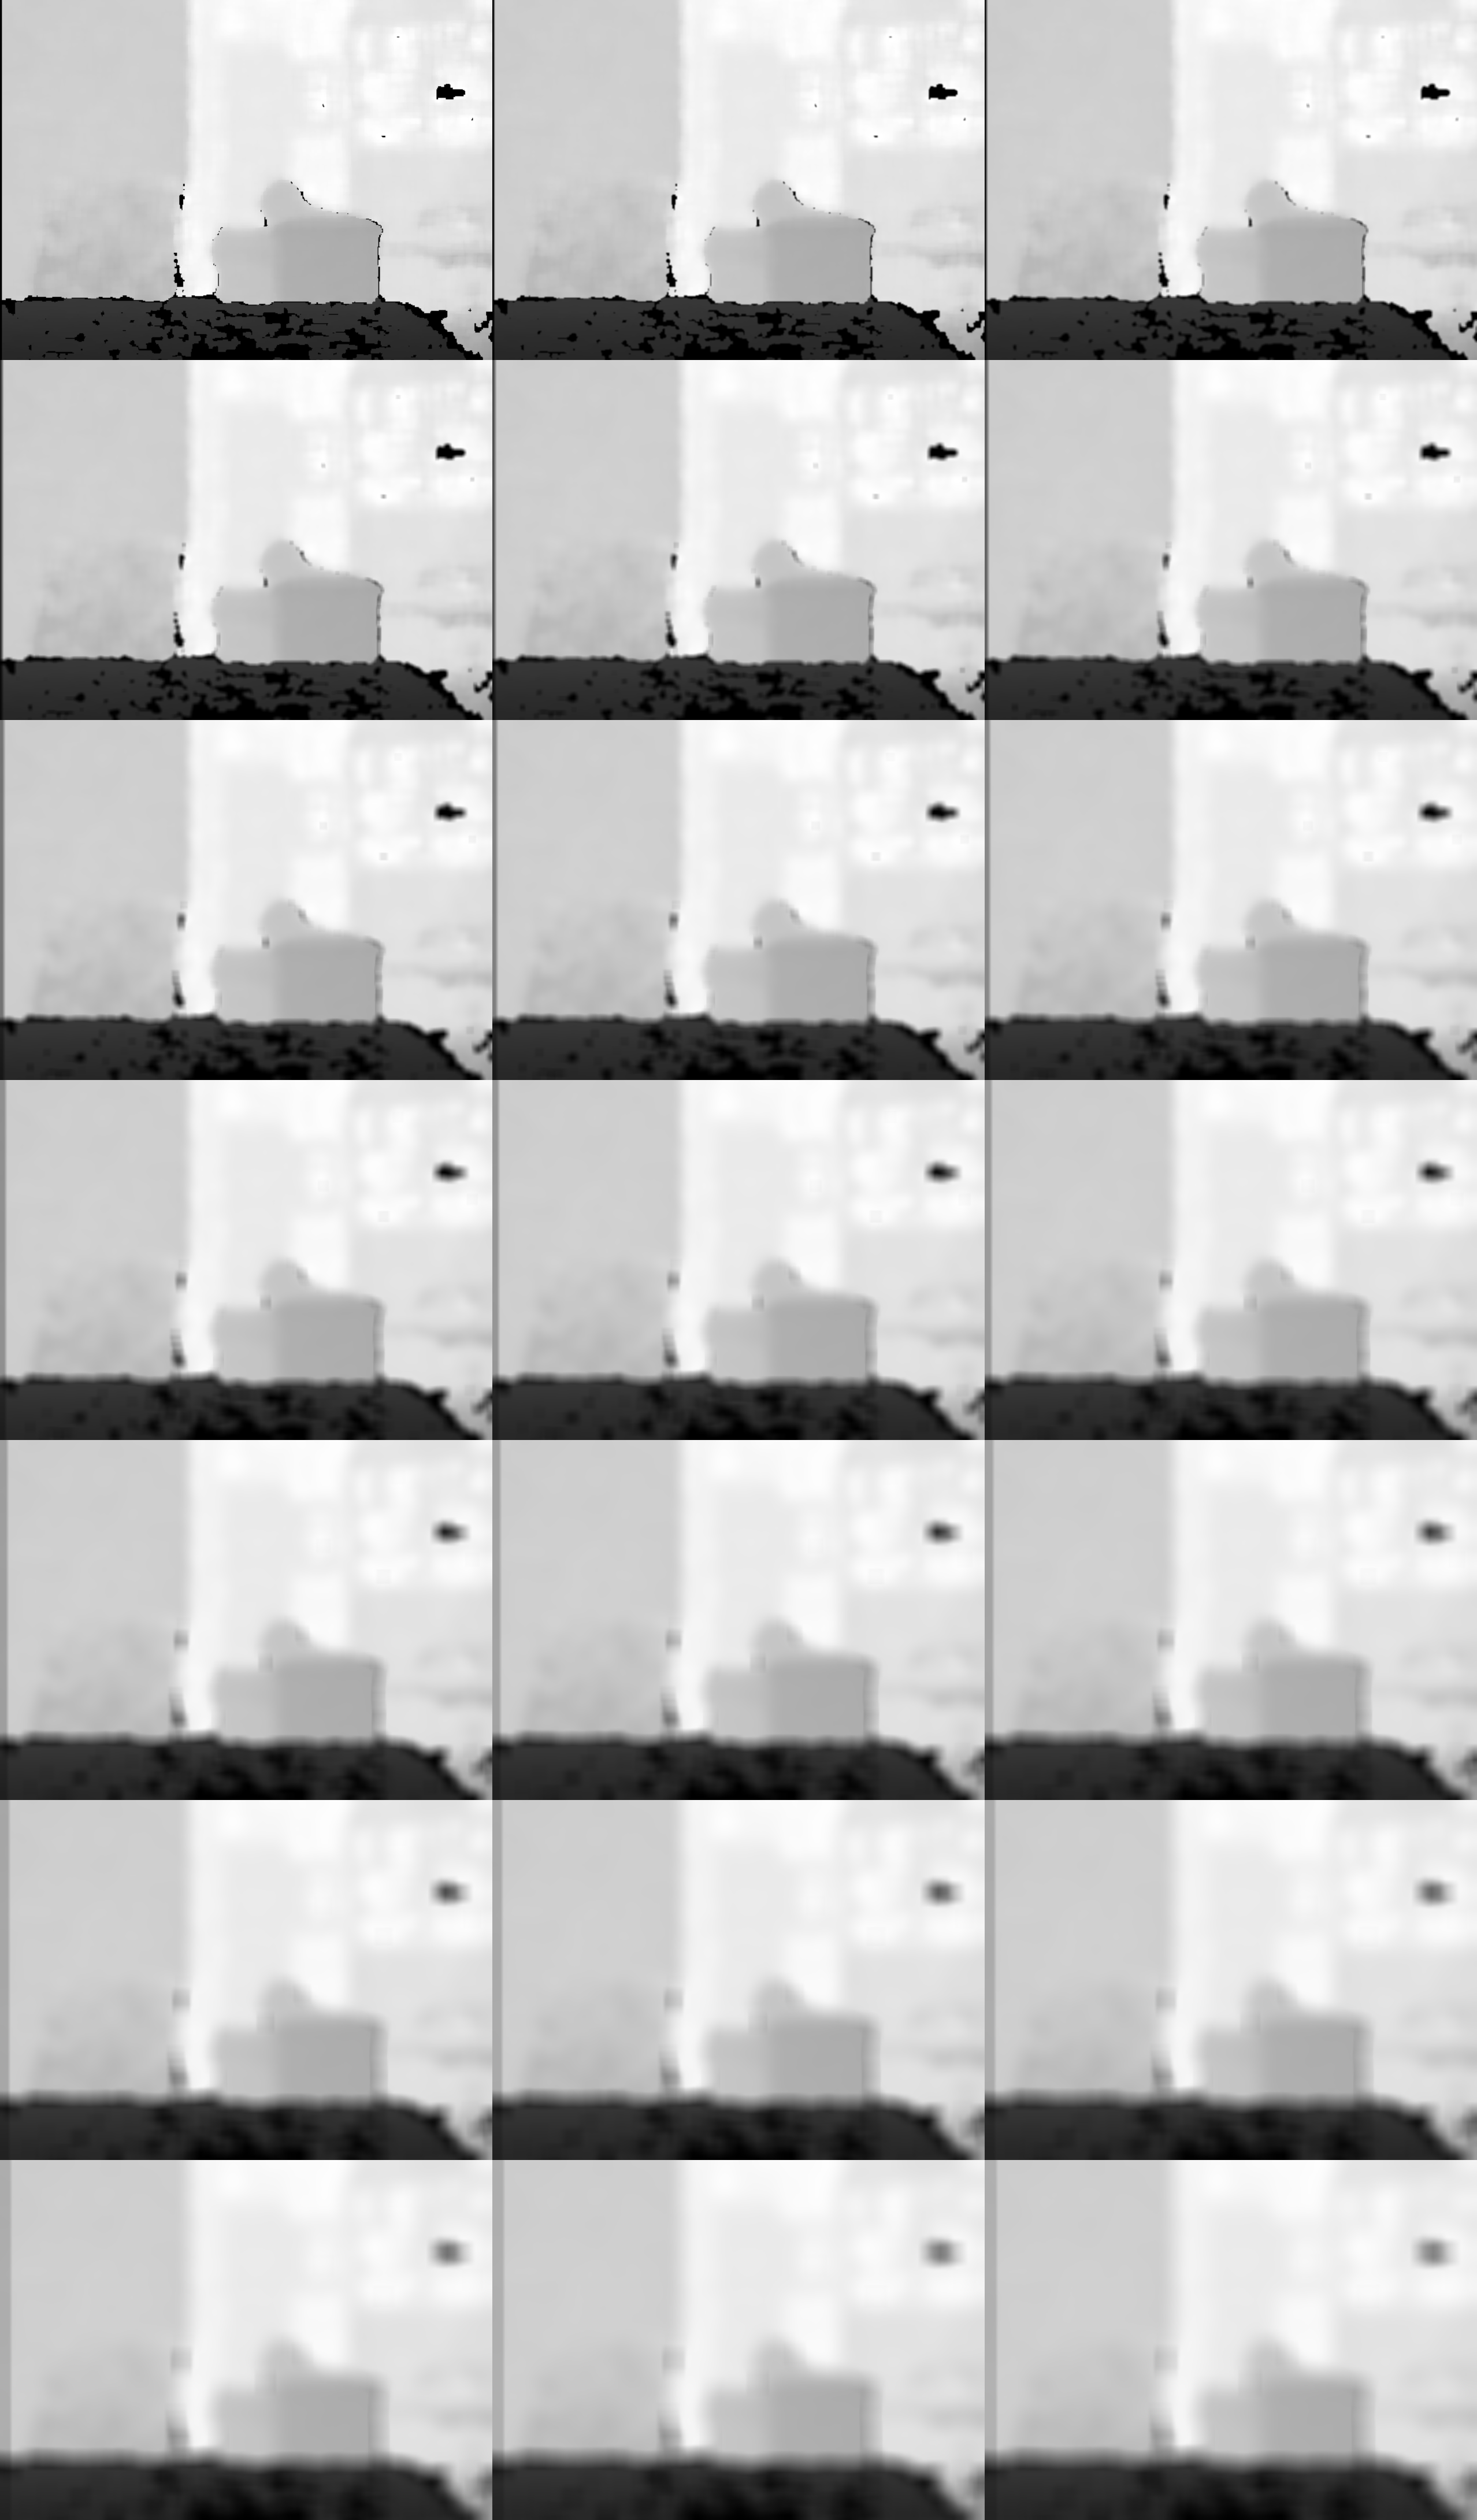
\includegraphics[width=\textwidth,height=0.9\textheight,keepaspectratio]{Images/blur/04_average_gray_grid.png}
		\caption{Averaging — Gray grid result}
	\end{figure}
	\clearpage
	
		\subsubsection*{Output (Colored Grid)}
	\begin{figure}[H]
		\centering
		\includegraphics[width=\textwidth,height=0.9\textheight,keepaspectratio]{Images/blur/04_average_colored_grid.png}
		\caption{Averaging — Colored grid result}
	\end{figure}
	\clearpage
	
	\subsection{Gaussian Blurring}
	\subsubsection*{Code}
	\inputminted{python}{Python_Files/05_gauss_blur.py}
	
		% Gaussian Blurring
	This blur uses a Gaussian kernel, giving more weight to closer pixels.  
	\textbf{Use:} Effective for removing Gaussian noise while keeping smoother transitions.
	

	
	\subsubsection*{Output (Gray Grid)}
	\begin{figure}[H]
		\centering
		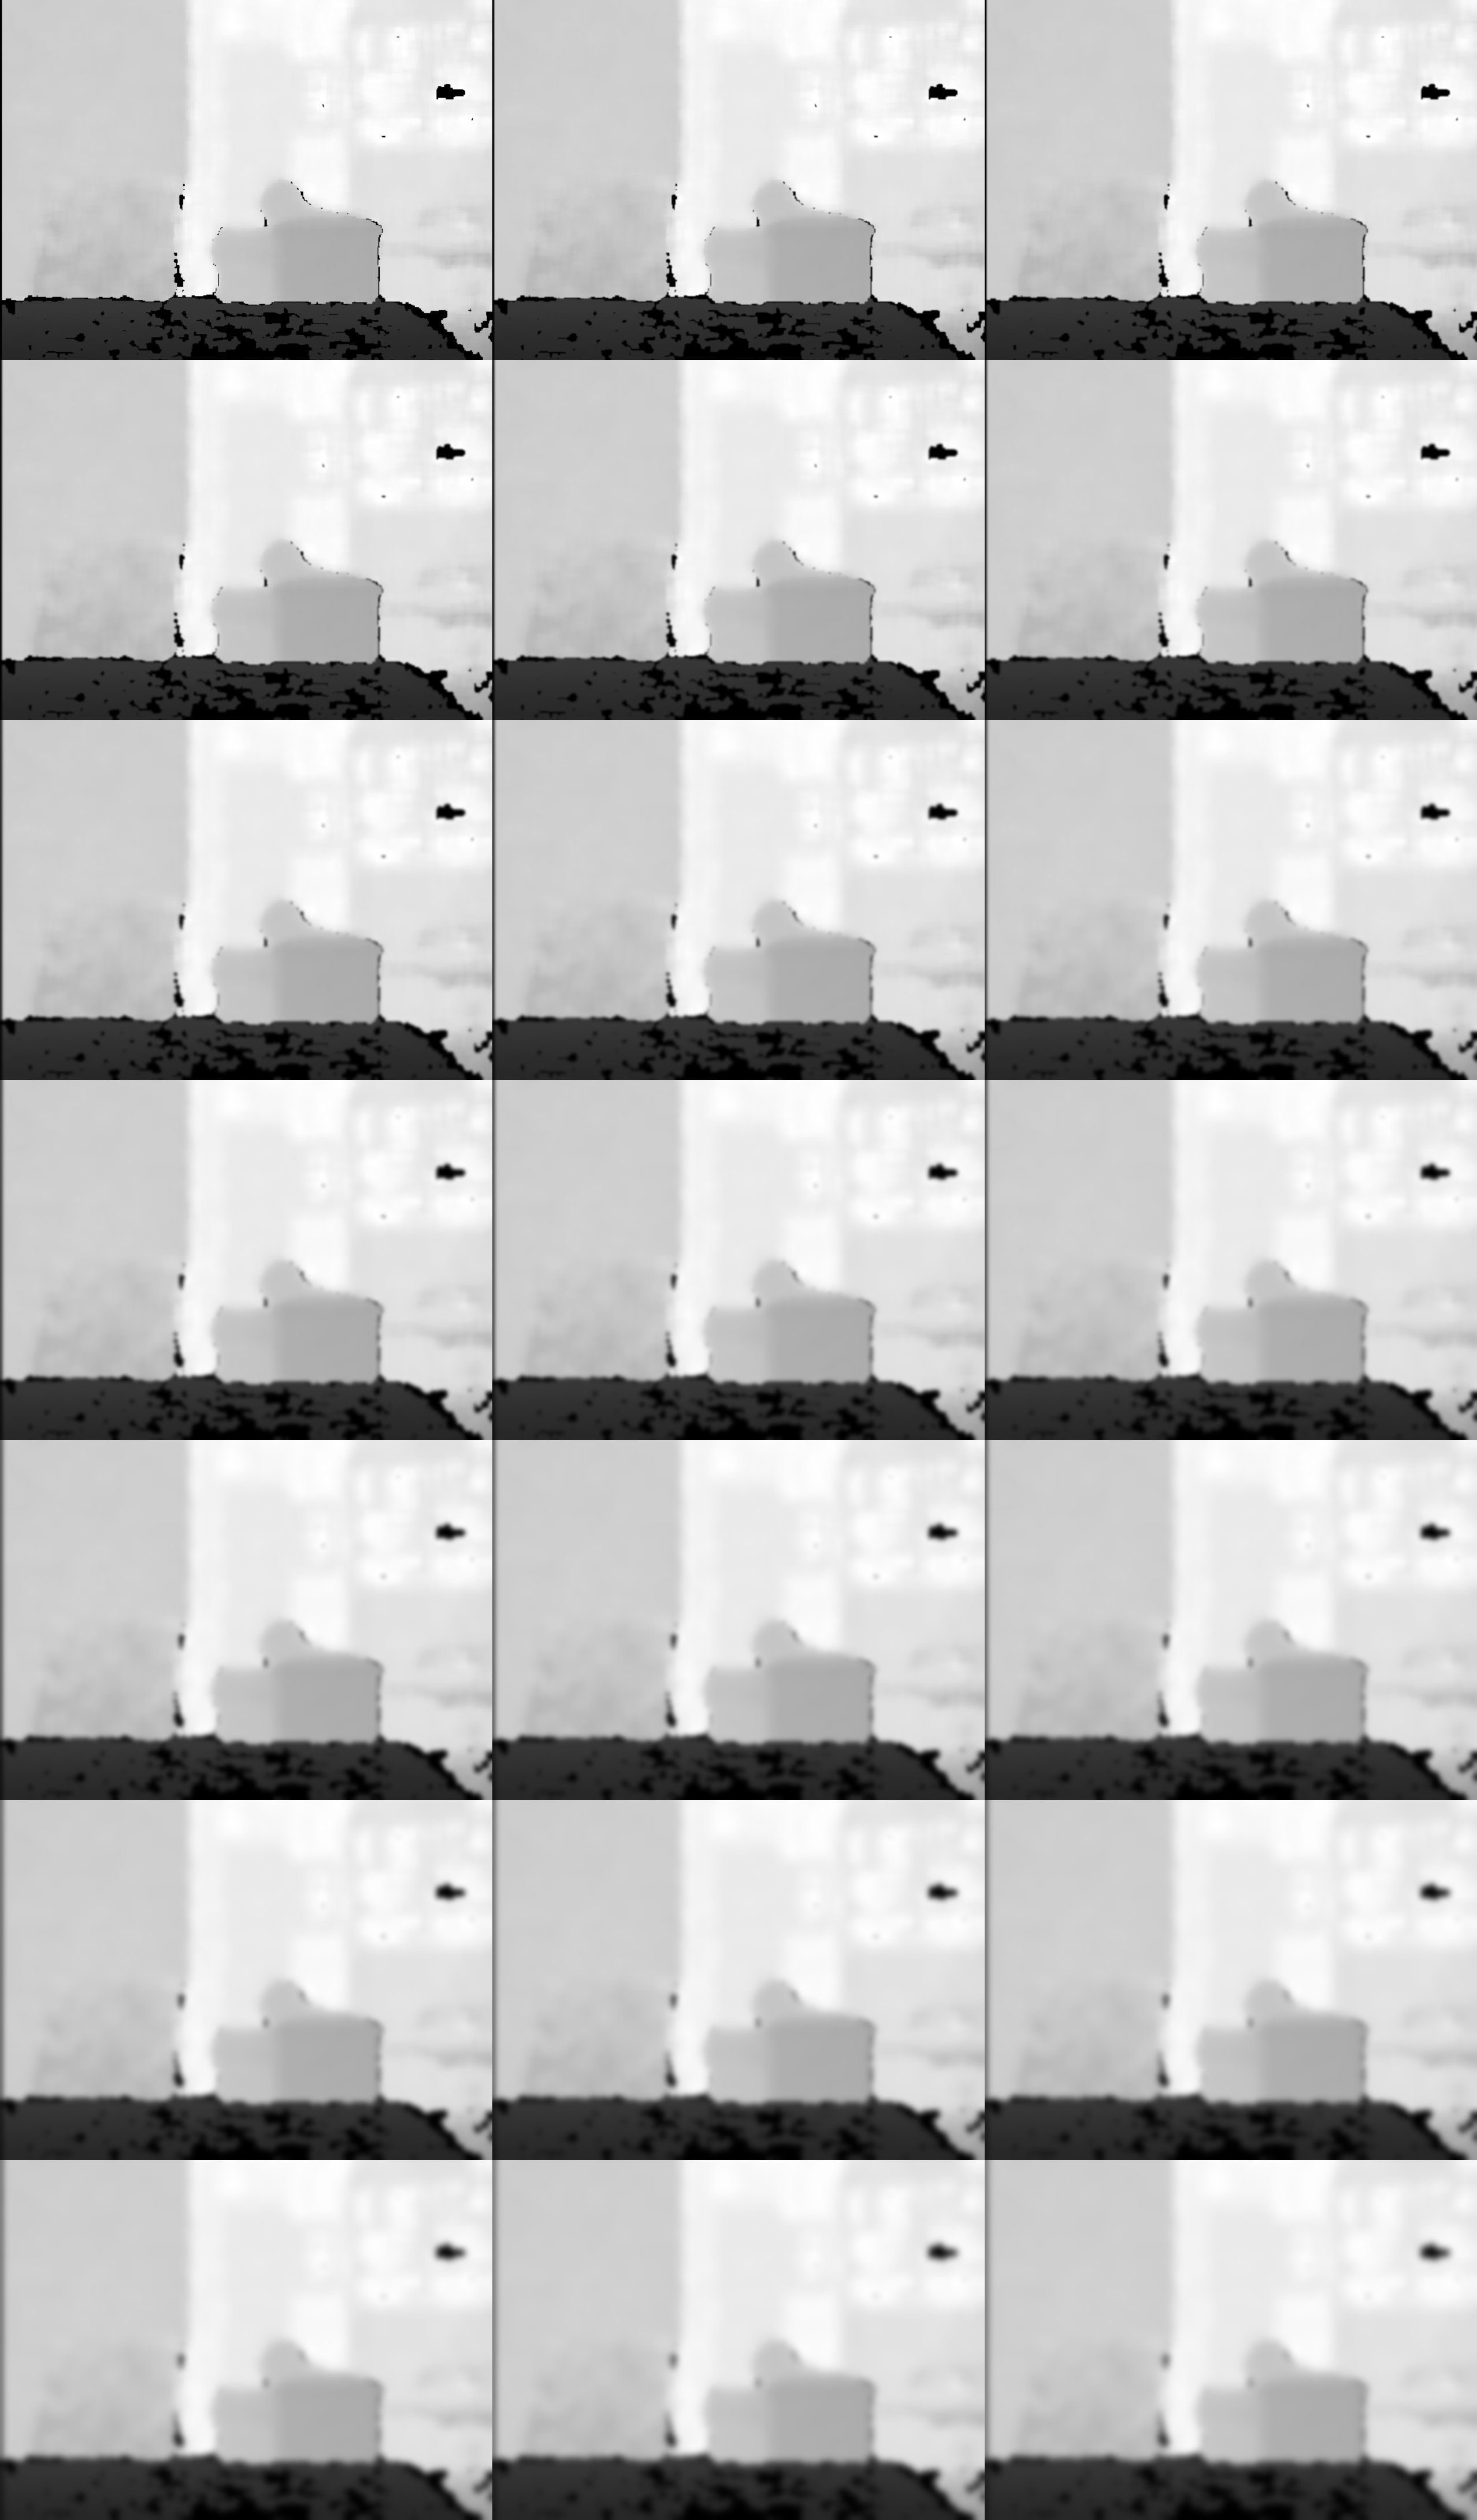
\includegraphics[width=\textwidth,height=0.9\textheight,keepaspectratio]{Images/blur/05_gaussian_gray_grid.png}
		\caption{Gaussian blurring — Gray grid result}
	\end{figure}
	\clearpage
	
	\subsubsection*{Output (Colored Grid)}
	\begin{figure}[H]
		\centering
		\includegraphics[width=\textwidth,height=0.9\textheight,keepaspectratio]{Images/blur/05_gaussian_colored_grid.png}
		\caption{Gaussian blurring — Colored grid result}
	\end{figure}
	\clearpage
	
	
	
	\subsection{Median Blurring}
	\subsubsection*{Code}
	\inputminted{python}{Python_Files/06_median_blur.py}
	
		% Median Blurring
	This blur replaces each pixel with the median of neighboring pixels.  
	\textbf{Use:} Very effective against salt-and-pepper noise, preserves edges better.
	

	
	\subsubsection*{Output (Gray Grid)}
	\begin{figure}[H]
		\centering
		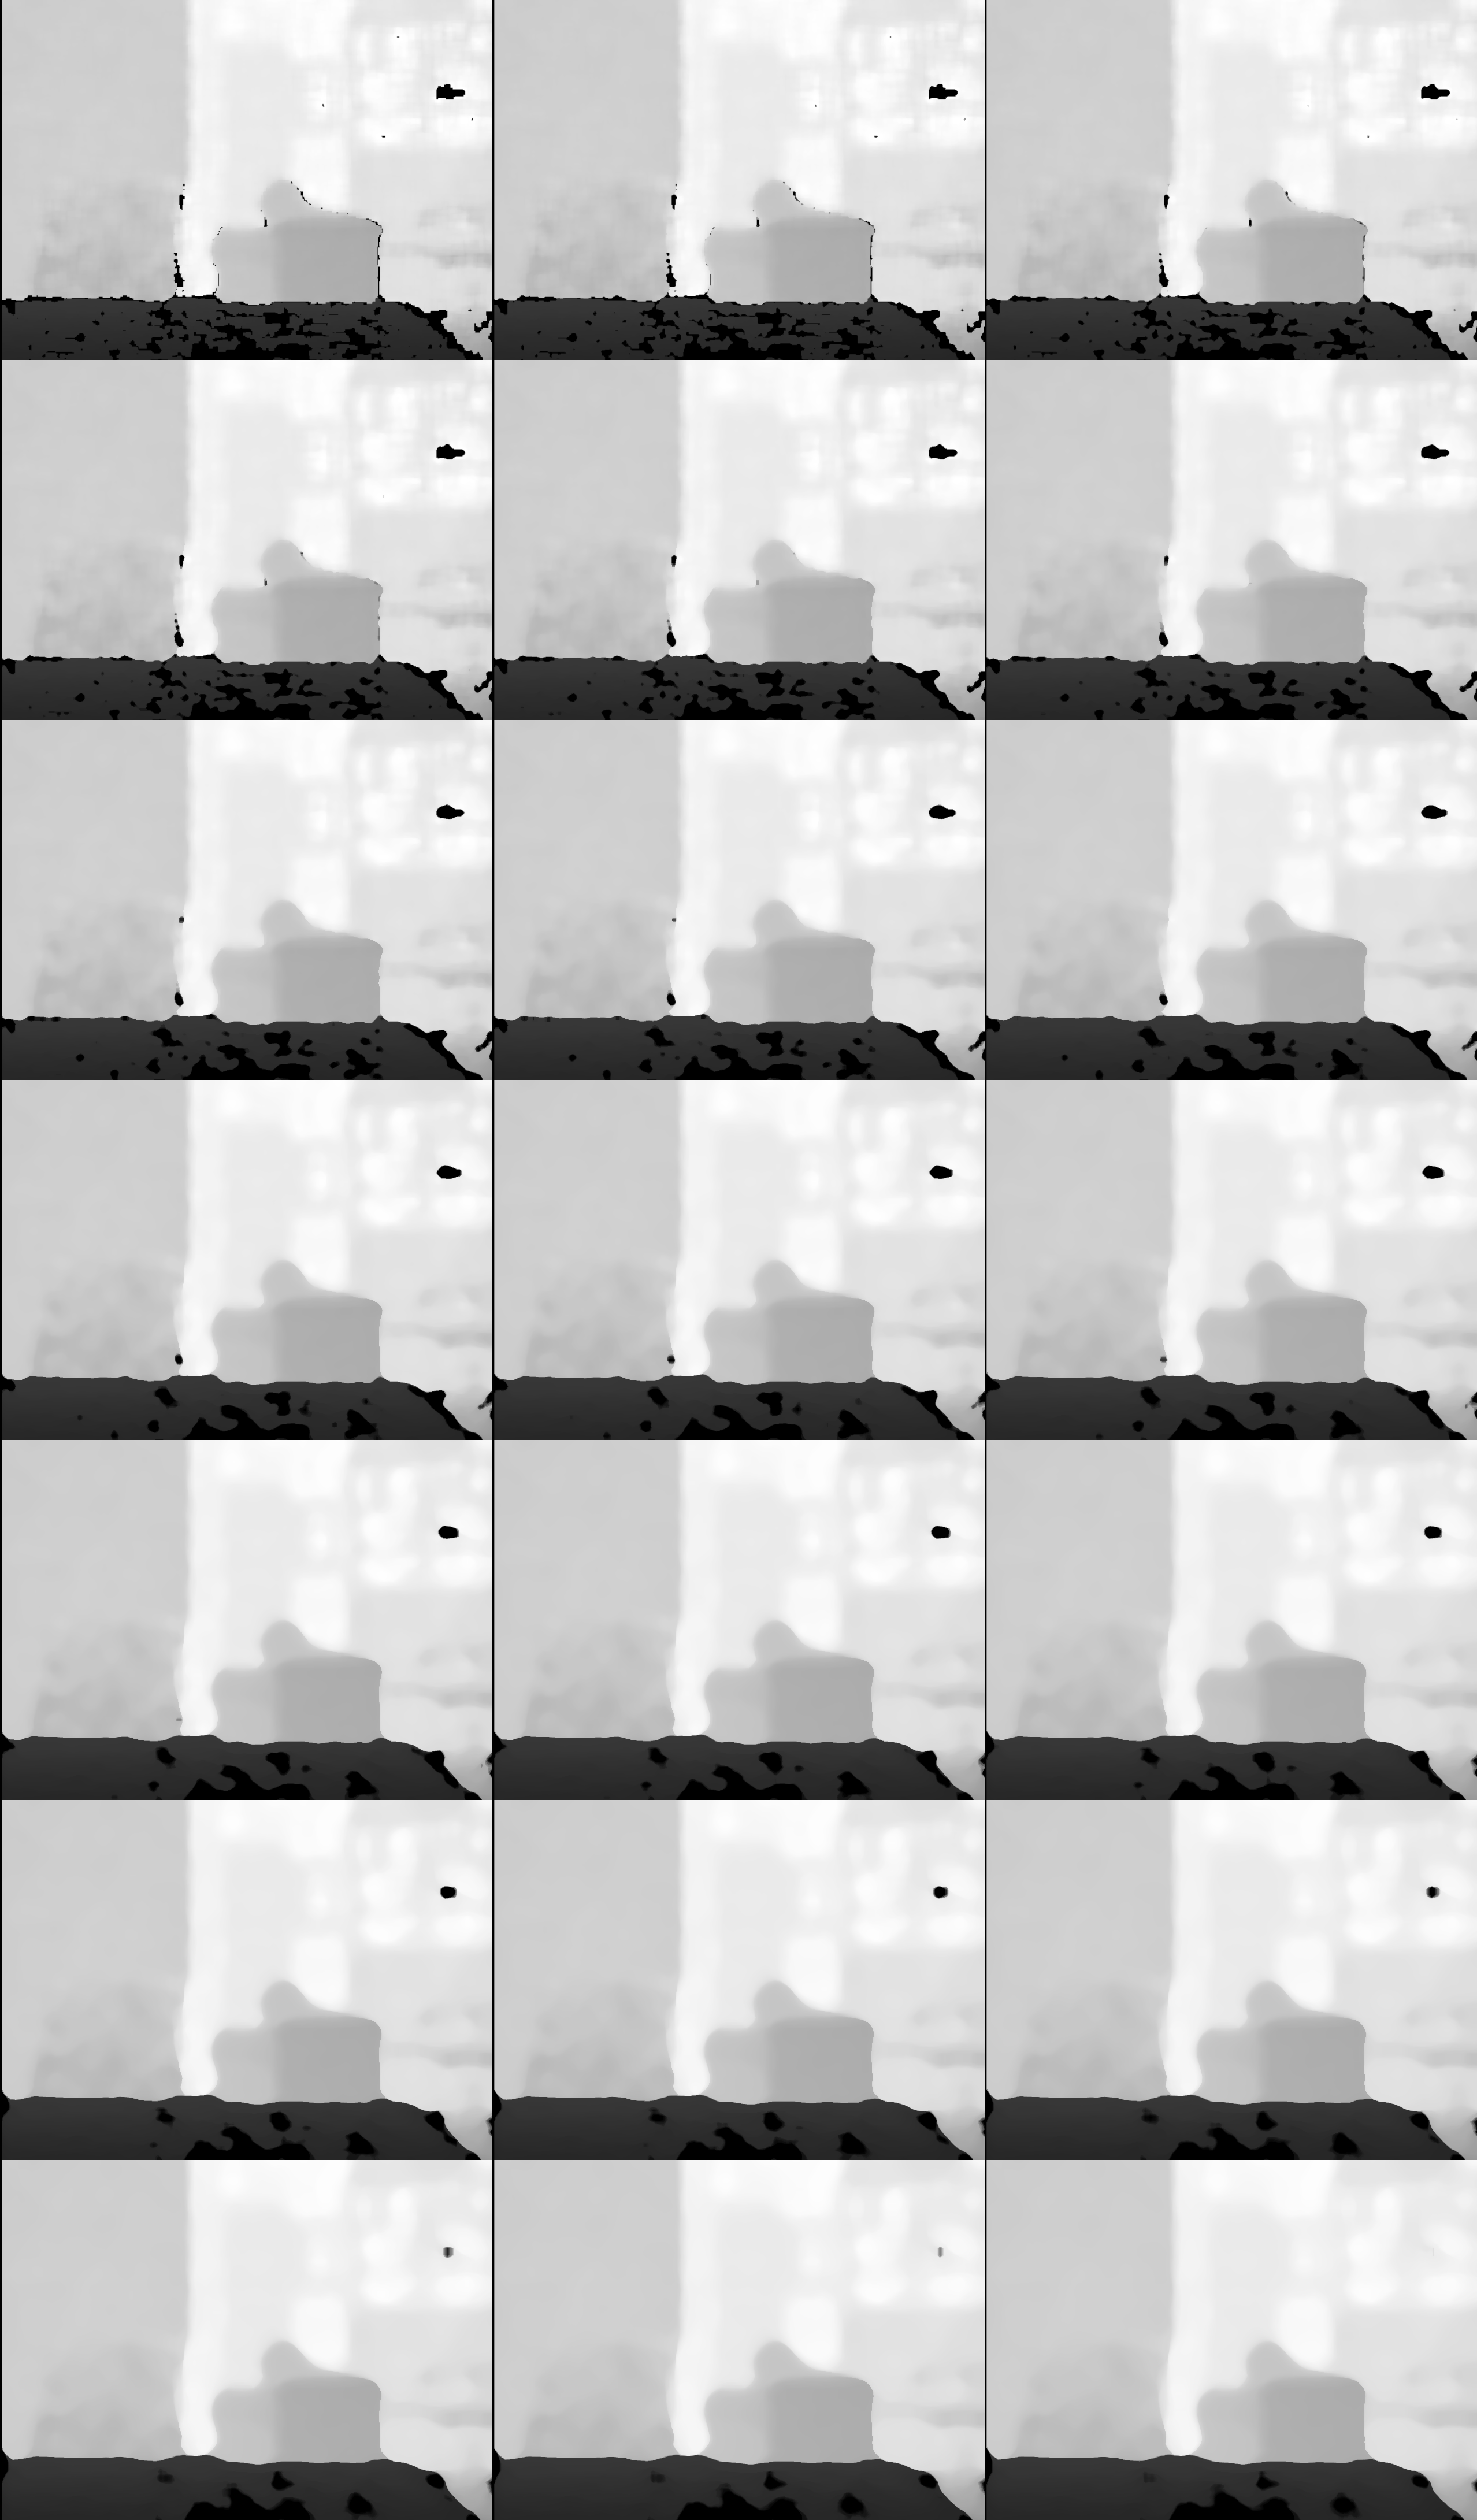
\includegraphics[width=\textwidth,height=0.9\textheight,keepaspectratio]{Images/blur/06_median_gray_grid.png}
		\caption{Median blurring — Gray grid result}
	\end{figure}
	\clearpage
	
	\subsubsection*{Output (Colored Grid)}
	\begin{figure}[H]
		\centering
		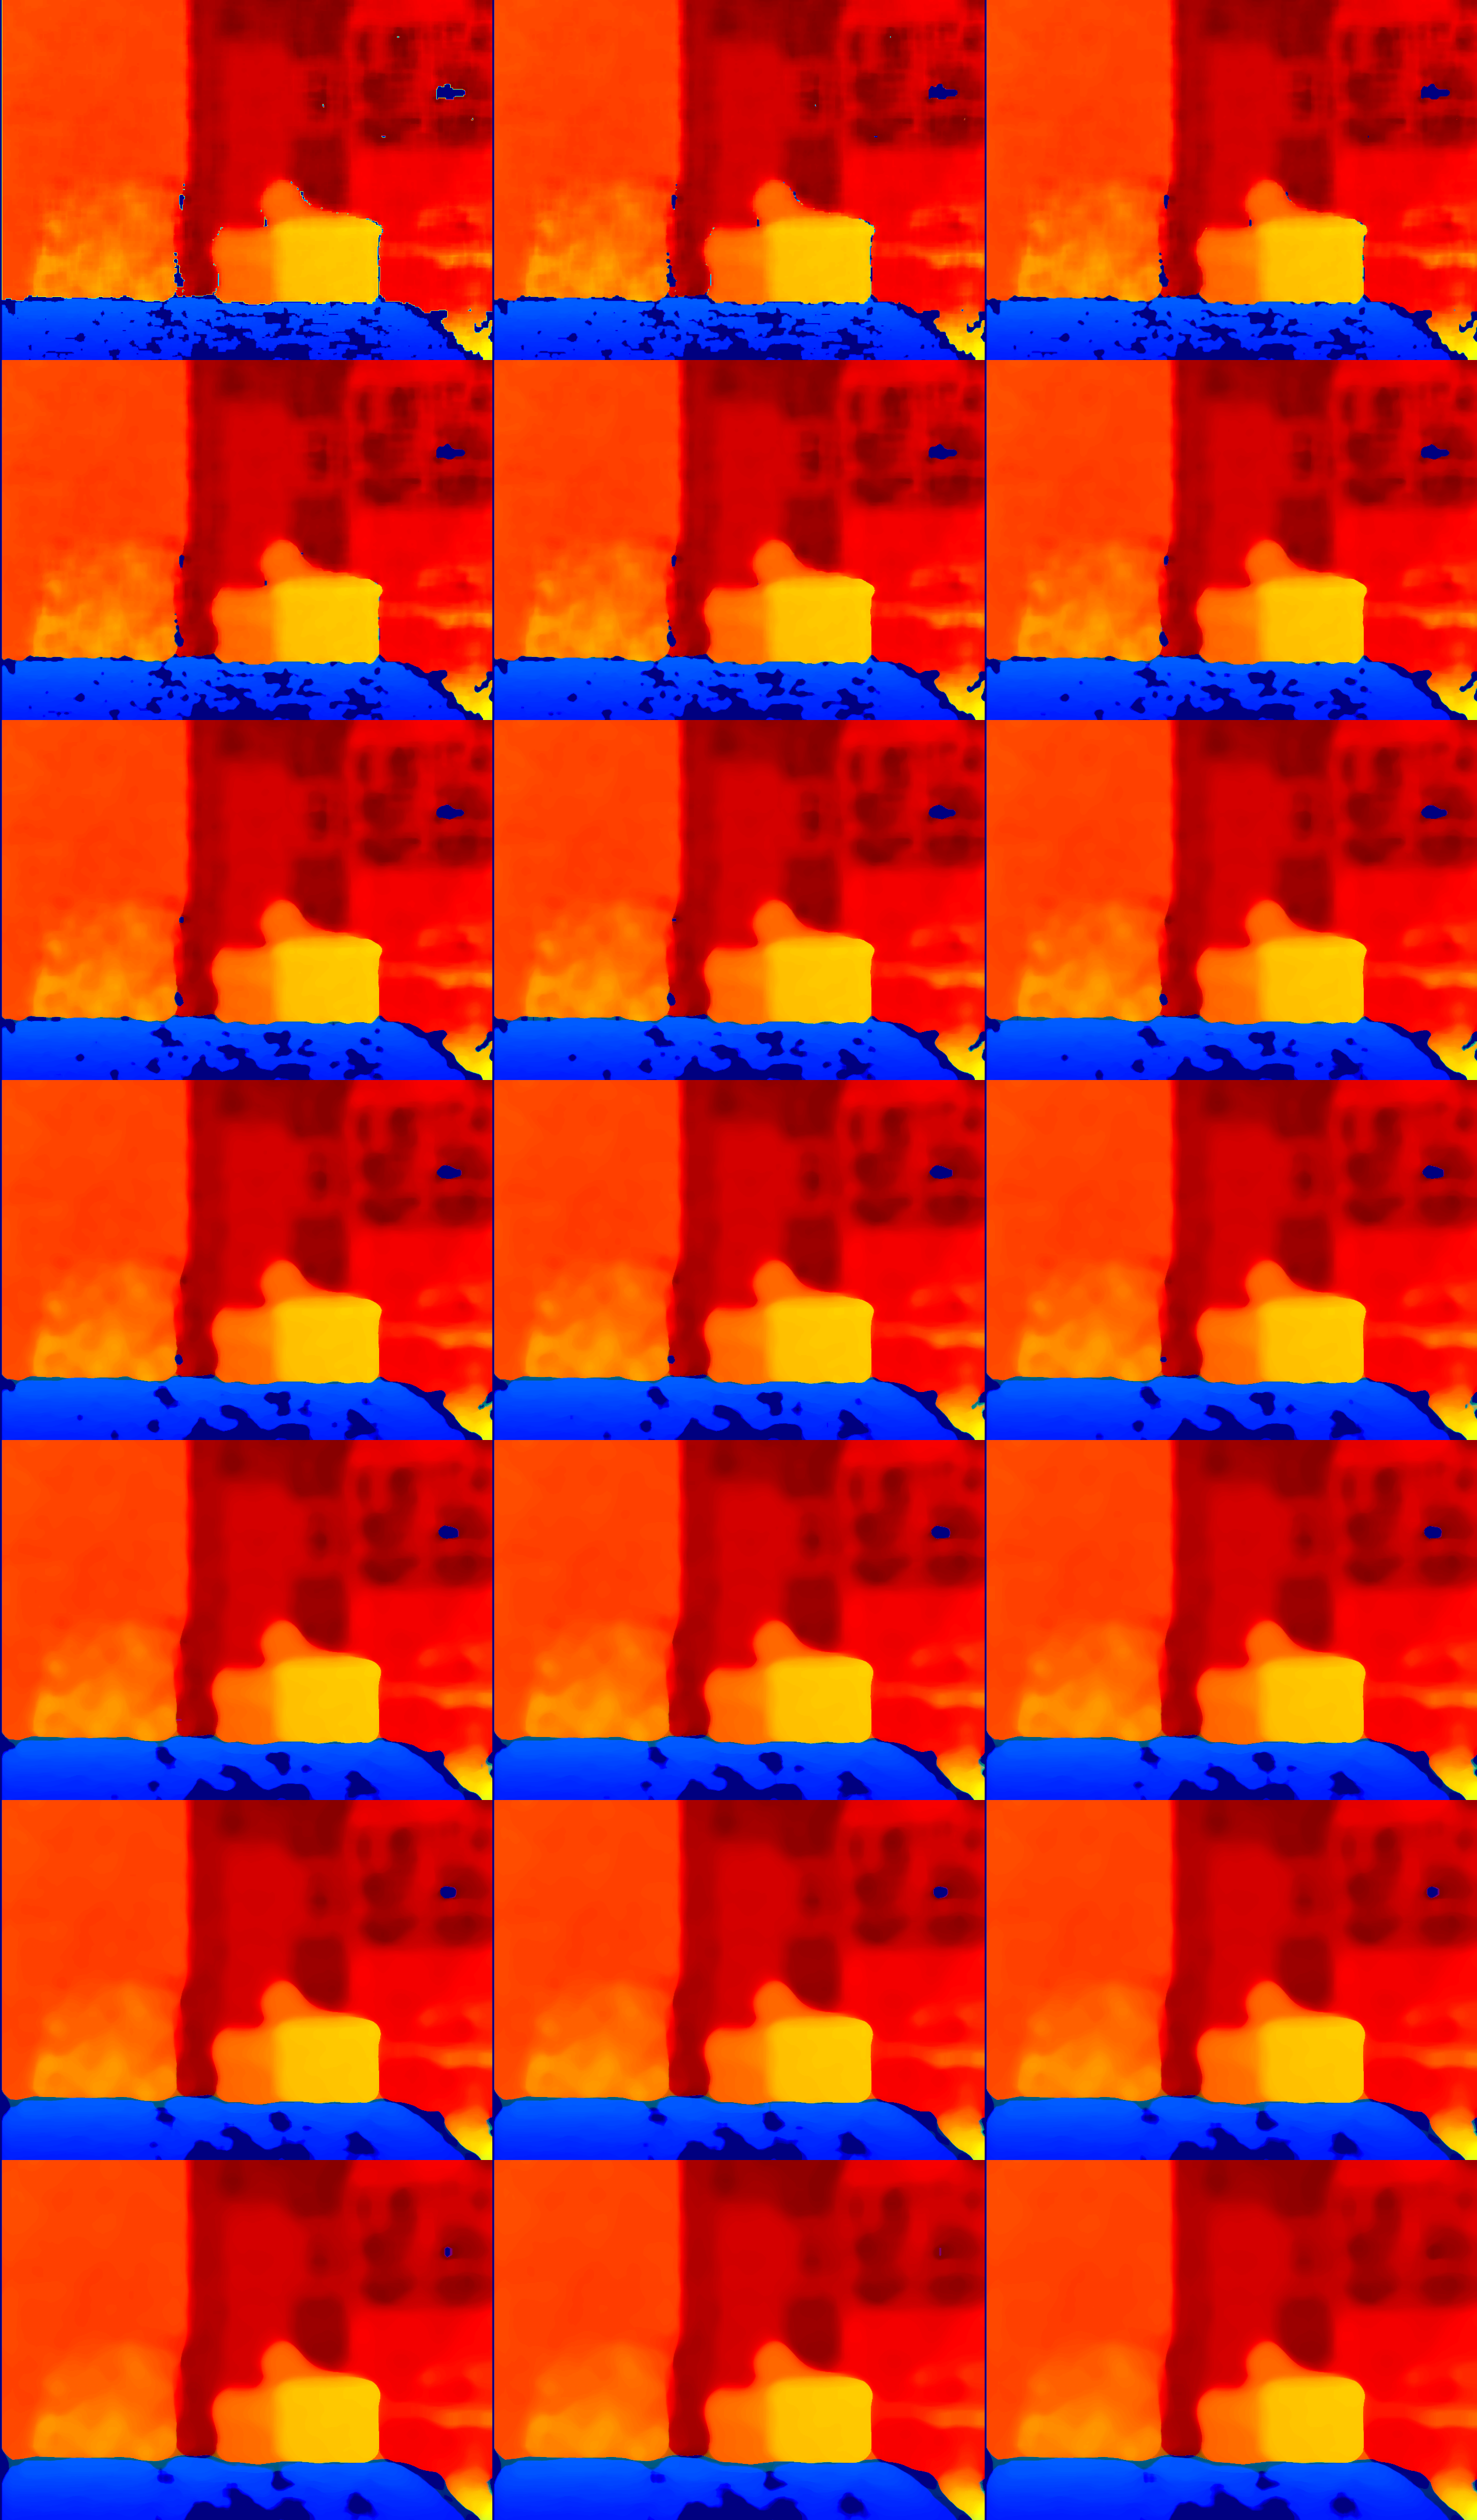
\includegraphics[width=\textwidth,height=0.9\textheight,keepaspectratio]{Images/blur/06_median_colored_grid.png}
		\caption{Median blurring — Colored grid result}
	\end{figure}
	\clearpage
	
	\subsection{Bilateral Filtering}
	\subsubsection*{Code}
	\inputminted{python}{Python_Files/07_bilateral_blur.py}
	
		% Bilateral Filtering
	This blur considers both spatial closeness and pixel intensity similarity.  
	\textbf{Use:} Removes noise while preserving sharp edges, but slower than others.

	\begin{figure}[H]
		\centering
		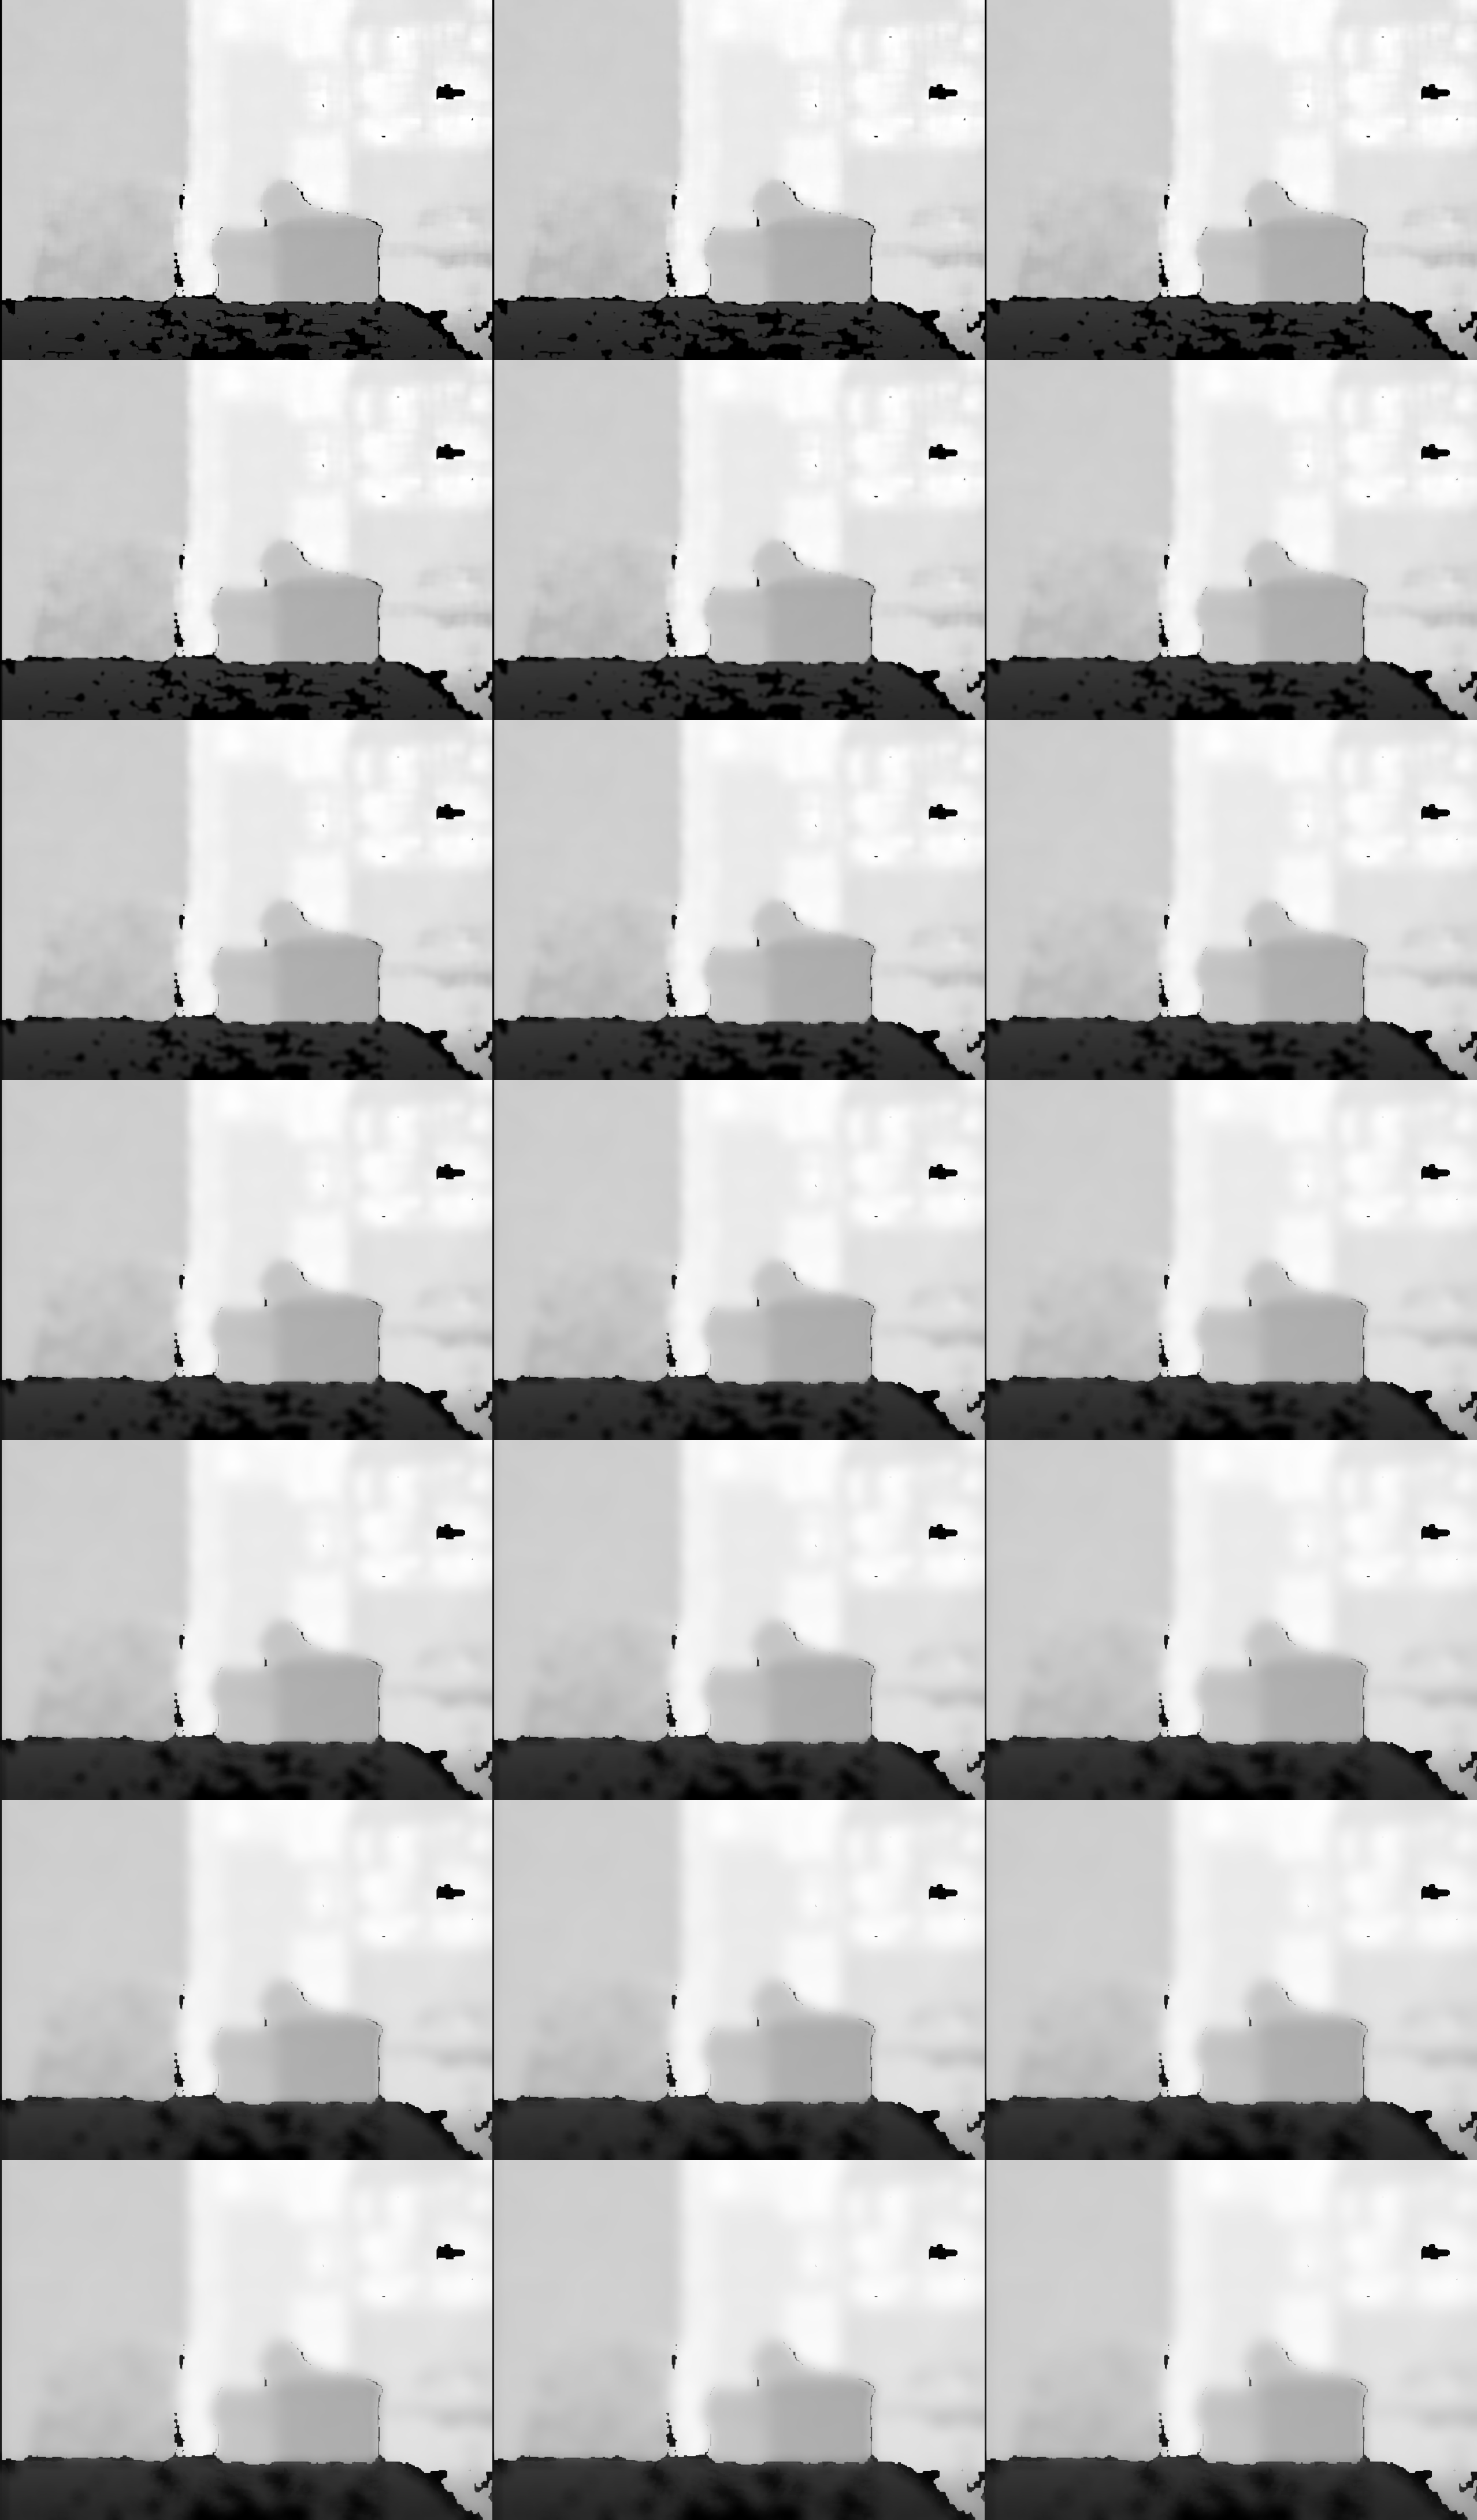
\includegraphics[width=\textwidth,height=0.9\textheight,keepaspectratio]{Images/blur/07_bilateral_gray_grid.png}
		\caption{Bilateral filtering — Gray grid result}
	\end{figure}
	\clearpage
	
	\subsubsection*{Output (Colored Grid)}
	\begin{figure}[H]
		\centering
		\includegraphics[width=\textwidth,height=0.9\textheight,keepaspectratio]{Images/blur/07_bilateral_colored_grid.png}
		\caption{Bilateral filtering — Colored grid result}
	\end{figure}
	
% Requires in preamble: \usepackage{graphicx,pgffor}


\section{Canny Edge Detection on Blur }

\subsubsection*{Code}
\inputminted{python}{Python_Files/08_canny_on_blur.py}

\PrintCannySeries{avg}
\PrintCannySeries{gauss}
\PrintCannySeries{median}
\PrintCannySeries{bilateral}


	
\end{document}
